\chapter{Background}
\label{chp:background}
This chapter looks at the literature around prostheses and locomotion mode selection 
% What are we interested in and why - understand what a healthy gait cycle is and how it changes for amputees
% Lower limb biomechaincs - terminology and what is the lost functionality after amputation
% How have prosthesis developed over the years
% Requirements for a prosthetic to replicate non-amputee/lost gait functionality - need to identify locomotive mode
% ML methods for classification of gait/locomotion mode
% What are the research gaps

How is this chapter structured



%---------------------------------------------%
\section{Biomechanics of Gait}
Gait is a highly individualistic personal trait with many factors that affecting it\cite{Horst2019}. A performant gait is a coherent highly energy-efficient mechanism for forward propulsion of the body. It naturally adapted to different environmental conditions and disturbances to achieve high level of stability throughout the gait cycle\cite{Shah2020, Mummolo2013}. With regards to lower-limb prosthetic the mechanics of locomotion are of most interest. Within this section the terminology that will be used to with reference to the human gait and the high level biomechanics of locomotion are presented.

\subsection{Gait Terminology}
% Key events in the gait cycle
A complete gait cycle is the basic unit of gait analysis. A cycle, by convention, begins when one foot comes into contact with the ground and is complete when the same foot contacts the ground again. This contact point is referred to as \acrfull{ic}, or more commonly \acrfull{hs} as this is the most common initial point of contact. Conversely the point at which the foot leaves the ground is referred to as \acrfull{to}. The name arises as the toe is always the last point of contact with the ground.\cite{Novacheck1998, Shah2020}

The gait cycle can be further sub-divided into two phases. The distinct phases, stance and swing, are physically indicated by the foots contact with the ground. Stance is when the foot is in contact with the ground, and swing the opposite, when the foot is off the ground. \acrshort{hs} marks the transition from swing to stance and \acrshort{to} stance to swing. When considering both limbs there are additional key events, Single Support when only one foot is in contact with the ground, i.e. in stance, and Double Support when both feet are in contact with the ground. Figure \ref{fig:background_gait_cycle} illustrates a complete gait cycle and the key events within it.\cite{Novacheck1998, Shah2020}

% Picture of gait cycle indicating key events
\begin{figure}[hbt!]
    \centering
    \includegraphics{example-image-duck}
    \caption[Full Human Gait Cycle]{Full Human Gait Cycle, \acrshort{ic} --- \acrlong{ic}, \acrshort{to} --- \acrlong{to}}
    \label{fig:background_gait_cycle}
\end{figure}

%Axis/Planes of human movement - Cardinal planes
Movements of the human body mostly occurs in three planes, Saggital, frontal/mediolateral and Horizontal/transverse. The intersection of these planes is either defined as the centre of the joint being studied or Center of Mass of the whole body. The Saggital plane is the vertial plane passing from rear (posterior) to the front (anterior), dividing the body into left and right. The frontal plane passes from left to right dividing the body into posterior and anterior halves. The horizontal plane divides the body into top (superior) and bottom (inferior) halves.\cite{Bartlett2007} Figure \ref{fig:background_planes_of_the_body} shows a illustration of the three planes.

\begin{figure}[!hbt]
    \centering
    \includegraphics{example-image-duck}
    \caption{Planes of human motion}
    \label{fig:background_planes_of_the_body}
\end{figure}

The major movement of the ankle occurs in the saggital plane, these are the raising and lowering the foot. The two motion are refereed to as plantar-flexion --- moving the foot downwards, and dorsiflexion --- lifting up the foot upwards.\cite{Bartlett2007}. Figure \ref{fig:background_plantar_dorsi_flexion} show a visual of the ankle movement. \hl{Add something about when each of these actions happens in a gait cycle{\cite{Whittle2012}} - pg40 onwards}

\begin{figure}[!hbt]
    \centering
    \includegraphics{example-image-duck}
    \caption{Saggital plane motions of the ankle. Plantar-flexion --- lowering the foot, Dorsi-flexion --- raising the foot}
    \label{fig:background_plantar_dorsi_flexion}
\end{figure}


%How is it measured (Cadence, stride length, toe clearance)/(Time and distance data)
There are many different metrics for quantifying gait. These vary from easily measurable values such as step rates and distances to more involved measures such as energy expenditure and efficiency. \hl{Some pertinent metrics to this area of research are; cadence --- the measure of gait cycle frequency}\cite{Ramakrishnan2019, Coutts1999}.


\subsection{Variation with Locomotive Activity}
% Introductory paragraph
The previous section described the pattern of gait that occurs during a level walking locomotion. The human gait cycle is able to efficiently adapt to different terrain and obstacles. In built up environments common locomotive activities include climbing stairs and walking up an down sloped surfaces. This requires a change in gait actions to accomplish the movement. Additional muscle actions are required to raise and lower the center of mass during these action\cite{Franz2012a}. 

Within this section the actions during four different locomotive movements are presented, \acrfull{sa}, \acrfull{sd}, \acrfull{ra}, \acrfull{rd}. Ramps are con sided any surface that has a slope sufficiently steep as to require a change in locomotive action. \hl{The differences are presented as evidence that of the variation in control modes that the human body employs.} % This needs some more work
The description of each of the actions is in comparison to level walking.

% Different locomotive modes (W, S, RA, RD, SA, SD)
\textbf{Stair Ascent} --- During \acrshort{sa} net positive work is required to move the \acrfull{com} upwards, this results in a greater muscle activity. \acrshort{sa} can be divided into three phases: weight acceptance, pull-up and forward continuation. During weight acceptance and pull-up the knee dominates with support of the hip and ankle. While, during forward continuation the ankle generates a large amount of energy - this is the point at which the  \acrshort{com} is pushed upwards. The ankle angle differs from horizontal walk mostly at the late swing phase and at the early stance. At the lift up to next staircase the edge is avoided by a small dorsiflexion and moving the knee backwards.\cite{Svensson2007} \hl{This is too similar to Svensson's original paragraph} 

\textbf{Stair Descent} --- During \acrshort{sd} the ankle angle differs from horizontal in the swing phase when moving the limbs down. This is most notable as a dorsiflexion to reach the toe downwards, leading to the toes being the point of IC. At this state most of the energy is transferred in the knee and ankle. At push-off a much smaller force is needed since the leg almost only has to fulfill the swing. Less muscle activity for vertical movements is also needed when descending due to the smaller stride length.\cite{Svensson2007}\hl{Again another citation would be good}

\textbf{Ramp/Hill Ascent} --- As with \acrshort{sa} during \acrshort{ra} additional energy expenditure is required to move the \acrshort{com} uphill\cite{Franz2012a}, walking uphill takes three times as much energy as walking on a flat ground\cite{Matsumoto2017} Gait parameters also vary systematically with the slope of the surface\cite{Kimel-Naor2017}. Knee flexion and ankle dorsiflexion increases at heel strike as the foot aligns with the surface. The variation require an increase range of motion and additional muscle power generation.\cite{McIntosh2006}

\textbf{Ramp/Hill Descent} --- For moderate slopes walking down hill is similar to level walking. However the lowering of the \acrshort{com} requires additional energy to be absorbed\cite{Franz2012a}, walking downhill takes only half as much energy as walking on level ground\cite{Matsumoto2017}.

%Concluding remarks
This all suggests that the nervous system uses different control strategies to adapt to different activities\cite{Lay2007} The adaptations that are automatically made to in a healthy gait cycle but must be made by any prosthetic controller to fully restore any lost functionality. This requires perceptive functionality to detective the intended action.

% Transition between activities of key importance
``Human activity recognition (HAR) is a hot research topic which aims to understand human behavior and can be applied in various applications. However, transitions between activities are usually disregarded due to their low incidence and short duration when compared against other activities, while in fact, transitions can affect the performance of the recognition system if not dealt with properly.''\cite{Li2019}

%---------------------------------------------%
\section{Prostheses}
Define a prostheses - Section introduction

%(Is this part of motivation in intro?)
Described amputation and it's prevalence - why is research in this area relevant 


Lower-limb amputation is the removal of a part, or multiple parts, of the lower limb. Though there is some discrepancy in literature regarding exact distal boundaries, it is generally accepted that “major” amputations include those which are at or proximal to the ankle.
Types of amputee -- trans-femoral - above knee, trans-tibial - below knee
According to the amputation level, lower limb amputation can be classified into toe, ray, transmetatarsal, mid-foot, below-knee (transtibial) and above knee (transfemoral) amputations

% Briefly can be talked about more in chapter 6
What are the differences/challenges in gait for amputees? 

%   - Asymmetry - left-right coordination and gait variability are robust characteristics of walking\cite{Kimel-Naor2017}
%   - Compensatory mechanisms \cite{Silverman2008}
%   - Reduced power generating muscles - decreases gait efficiency
%   - for non-amputees these changes between activity are automatic sub-conscious
In the absence of ankle plantar flexor power, hip extensors and flexors as well as hip external rotators became the major power generators, whereas hip abductors and adductors and knee extensors muscle powers became the main source of absorption. For the sound limb, increased hip extensor activity was observed, accompanied by less hip abduction-adduction activity.\cite{Sadeghi2001}

Amputee gait is asymmetrical and different from that of able-bodied individuals, amputees relying more heavily on their unaffected side.\cite{Bateni2002, Varrecchia2019}

What is the aim of prosthetic devices - to restore the lost functionality of the limb - \cite{Tucker2015}


% ----------------------------------
\subsection{History of Prosthesis}
History of prosthesis

Traditionally mechanically passive

cannot provide the net positive mechanical power needed during many activities of daily living, such as ascending stairs or standing up from a seated position\cite{Simon2013}.

What is current state of the art (Powered prosthesis)



% ----------------------------------
\subsection{Control requirements} % Introduce the problem
The human body represents a well-balanced walking machine that performs periodic, stable, and energy-efficient gait through highly sophisticated mechanics and control, which are not easily replicable\cite{Mummolo2013}

Powered prosthesis require control to ensure they work in unison
% Volitional vs Automatic movement

Different control modes are required for different activities\cite{Simon2013}

What are the control requirements - high level(perception) $\rightarrow$ low level\cite{Tucker2015}




%---------------------------------------------%
\section{Sensors} % THIS IS COPIED FROM TRANSFER REPORT - NEEDS UPDATING!
Perceived intent must be inferred through quantitative measurements of the user and their environment. Appropriate selection of sensors is therefore of critical importance requiring consideration of the type and richness of the information they provided as well as the impact they have on the user.\cite{Tucker2015}

Impact is described by its invasiveness which is ``the relative ease (in time, effort, and risk) with which a sensor may be applied and removed''\cite{Tucker2015}. As an example a surgically implanting electrode is highly invasive whereas a sensor placed on a prosthetic limb is non-invasive.

Impact on a subjects gait due to the sensors or other additions is also of importance. Heavy or uncomfortable sensors are likely to affect gait, for example a sensor on shoe of less than 300g does not affect gait significantly\cite{AbdulRazak2012} whereas a large number of wires rubbing on the leg may.

Sensing systems can be divided in to three categories, those that measure neural, mechanically intrinsic or environmental signals. Neural sensors tap into physiological electrical signals, such as brain activity or muscle activity. Mechanically intrinsic sensors measure effects that are intrinsic to the device itself, such as acceleration. Environmental sensors measure properties of the world around them, ambient light for example.\cite{Koller2018, Tucker2015}

Neural sensors detect muscle control signals conversely mechanically intrinsic measure the effect of muscle force. Neural signals can therefore be detected earlier, 10s of milliseconds\cite{Tucker2015}, giving longer to perform classification although their output is often challenging to interpret. Mechanical signals are often simplier owing to their less invasiveness nature and greater tolerance to placement and conditions.\cite{Koller2018}

Gait analysis is traditionally a lab based activity requiring specialist facilities to capture data\cite{LeMoyne2017}. In this environment sensor portability is not normally a concern allowing the use of more permanent and sophisticated sensor systems. In contrast wearable sensors and data loggers must be small and light weight presenting a greater challenge to getting comparable readings. They have however the distinct advantage of being portable, facilitating measurements in a more natural environments\cite{Shull2014}.

In general new sensor packages are usually validated against lab equipment, with the result often used as a performance metric. For gait events this is often presented as a relative time offsets from the true occurance \cite{Greene2012, Lin2014, Doheny2010, Bejarano2015, Patterson2012}.

%=======================================%
\subsection{Placement}
Placement of sensors is an important consideration, they need to be located to maximise the richness of there data while minimising invasiveness\cite{Tucker2015}. Shull et al (2014) performed a review of the location wearable sensors for gait analysis, the majority of articles identified used sensors sensitive in medio-lateral axis, with the knee, trunk and shank the most popular sensing location. See Figure \ref{fig:ch3_shull_wearable_sensor_position}.

\begin{figure}[hbt]
    \centering
    \includegraphics[width=0.6\textwidth]{example-image-duck}
    \caption{Target gait parameter locations for wearable sensing, the number of articles reporting gait parameter locations is indicated at each respective location. The relative proportion of kinematic and kinetic parameters about each of the three anatomical axes is indicated in the pie charts. Adapted from \cite{Shull2014}}
    \label{fig:ch3_shull_wearable_sensor_position}
\end{figure}

For foot plantar pressure sensors the location of the foot sensor dictates which part of the stance phase it is sensitive to. In order to fully cover the foot 15 sensors are required\cite{AbdulRazak2012}, see Figure \ref{fig:lit-rev_foot_anatomical_area}, most studies use far fewer.

\begin{figure}[hbt]
    \centering
    \includegraphics[width=0.6\textwidth]{example-image-duck}
    \caption{Foot anatomical areas, heel (area 1-3), midfoot (4-5), metatarsal (6-10), toe(11-15)\cite{AbdulRazak2012}}
    \label{fig:lit-rev_foot_anatomical_area}
\end{figure}

For electrode based measurements the Surface ElectroMyoGraphy for the Non-Invasive Assessment of Muscles (SEMNIAM) project provides a standard for locating EMG sensors. Locations have been selected to provide a clear and stable EMG reading and allow comparable measurements between studies following the guidelines.\cite{Seniam}.

%Gyro locations\cite{Patterson2012} Sztyler et al 2017 also  a wide variety of accelerometer sensor placement locations identified shin and waist as best location for activity detection\cite{Sztyler2017}.

For prosthetic users the prostheses is the obvious mounting location providing a rigid and stable sensor platform. For biological limbs attachment is more challenging, attachment is usually performed using medical tape or elastic strapping. The changing shape of the limb during movement must also be considered.

%Type of data, information it provides, i.e. features, ways people have collected it.
%=======================================%
\subsection{Mechanically Intrinsic Sensors}
Angle, angular velocity and force/moments are the most commonly measured mechanically gait signals. A wide variety of wearable and grounded sensors can be used to collect this information.\cite{Shull2014, Tucker2015}

The most common wearable sensor used in is the Inertial Measurement Unit (IMU)\cite{Shull2014}. These often comprise of a 3-axis accelerometer, 3-axis gyroscope and 3-axis magnetometer as a single Integrated Circuit (IC). Using one or multiple sensors allows determination of limb or joint orientation, angular velocities and accelerations.
 
Other common wearable sensors include Goniometer/inclinometers, for angular displacements, and pressure transducers/Force Sensitive Resistors (FSR) for foot loading and initial/terminal contact points. Pressure transducers can be used to determine Ground Reaction Force (GRF)\cite{Schepers2007}. Where FSRs or other threshold sensors are used to detect gait features the detection threshold is of critical important\cite{Sabatini2005}. The value selected introduces a potential systematic bias into the results. Joint force or moments can be measured using various force sensors, for a prosthetic this can be achieved by instrumenting the shank tube\cite{Schepers2007}

Mechanomyography (MMG) can be used to estimate the force production in muscles by measuring sound or vibrations evident of the skins surface using microphones or accelerometers. They have a high sensitivity to motion artefacts so require a large amount of processing to extract a usable signal. Changes in muscle hardness or volume can also be used to estimate force.\cite{Tucker2015} Martin et al (2018) demonstrated how measurements of shear wave propagation through a tendon can also be used estimate joint torques. Shear waves are induced by tapping the tendon with a ultrasonic sensor used to the resultant signal\cite{Martin2018}.

In laboratory environments sensors generally include motion-capture systems and force plates. Motion capture allow millimetre accurate tracking of the user within the cameras range. Floor mounted force plates are used to measuring GRF, the user is required to time their walk so a step is taken on the plate and the plates are usually only large enough to measure one or two consecutive gaits.

%=======================================%
\subsection{Neural Sensors}
Neural signals provide a more natural interface for controlling prosthetics but pose significant challenges in there use. ElectroMyoGraphy (EMG) is the most common technique, electric potential produced by skeletal muscle activity is measured through electrodes attached to the muscle on interest.

Where suitable muscles are present at the skin electrodes can be attached to the skins surface above the muscle. Surface EMG present the least invasive technique for neural sensory system however they must be attached securely to the body to prevent artefacts from sensor movement corrupting readings and require individual calibration. Where amputation removes muscles surgical techniques can be performed.

A technique called Targeted Muscle Reinnervation (TMR) can be used to surgically reattached  severed nerves to a foreign muscle so they can be later used for EMG recording. This technique is most commonly used for prosthetic arms\cite{TMR2018}. Hargrove et al (2013) demonstrated this technique recording EMG data from severed nerves reattached in the stump resulting in a 10\% classification improvement with no critical errors occurring.\cite{Hargrove2013}. Srinivasan et al (2017) recently demonstrating an alternative technique that added a feedback path through the use of a agonist-antagonist muscle pair. The muscle pair provides a bi-directional myoneural interface allowing a closed loop control system to be completed with the central nervous system.\cite{Srinivasan2017} 

Koller et al (2018) compared a myoelectric controller to a equivalent mechanical intrinsic system for an lower limb exoskeleton, there was no measured difference in metabolic energy but subjects showed significantly less soleus muscle activity when using the mechanical systems. Koller concluded that as subjects weren't requred to engage the soleus they didn't. This suggest that equal performance can be obtained through either sensor form\cite{Koller2018}.

Kannape et al 2014 demonstrated a volitional control system, using the BiOM ankle, that allowed the user to control the amount of push off torque proportionally to the measured EMG signal from the Gastrocnemius muscle. The controller was tested for stair ascent, descent and level walking achieving good performance.\cite{Kannape2014}.

%% Prosthetic arms and upper limbs use these features more extensively
%Intracortical electrode arrays have been successfully demonstrated to allow control of multi-degree-of-freedom reach and grasp movements with robotic arms in tetraplegic subjects\cite{Tucker2015}.

Researchers have investigated the use of ElectroEncephaloGraphy (EEG) to measure brain activity. So far systems still place a high cognitive demand on the user are require extensive training as well as being highly susceptible to movement artefacts.\cite{Tucker2015}

%=======================================%
\subsection{Environmental Sensors}
The environment around the user can provide context to local sensor data. Different environments increase the likelihood of encountering a particular terrain feature.\cite{Tucker2015} Below different environmental sensors are briefly discussed with their usage discussed further in Section \ref{sec:lit-rev_enviroment}.

Only one paper by Zhang et al (2011) was found that presents use of environmental sensors for detecting locomotion mode. A laser distance sensor was used to scan terrain with a IMU used to calculate it angle. The measurements were used to calculate the height of terrain and it's horizontal distance from the user. Two locations for the sensor were tested, the shin and hip. Data from the shin was very susceptible to motion artefacts during swing.\cite{Zhang2011}

Jin et al (2014) investigated a wearable environmental sensing package to augment other methods for activity and location recognition. Three sensors were evaluated temperature, humidity, and ambient light. They measured repeatable changes in sensor data during different activities, for example a temperature drop due to airflow over the sensor package during motion.\cite{Jin2014}

Positioning methods based off no external reference, commonly known as dead reckoning, have been investigated by multiple authors. The use of a foot mounted IMU double integrating accelerometer to track position is the most common. Susceptibility to drift errors due to accumulating quantisation errors is the key challenge in this technique. Correction can be achieved by assuming foot is stationary when on the ground.\cite{Yun2007, Nilsson2014} Simultaneous Locating And Mapping is another common method, however this is very computationally intensive.


%---------------------------------------------%
\section{Machine Learning} % Big section on theory and application of machine learning
% Overview of machine learning aim and operation
\acrfull{ml} is a subset of computer science that focuses on systems that learn from data. An \acrshort{ml} system can numerically estimate a complex function from exposure to examples of a phenomenon. That is to say, an \acrshort{ml} algorithm can convert experience into expertise or make predictions from data. The numerical nature is especially compelling for problems of high dimensionality. What separates machine learning from optimisation is that we want to minimise the task error not only for the seen experience but also for novel unseen inputs. Minimising the task error forms the crux of machine learning.\cite{Mitchell1997, Shalev-Shwartz2014, Goodfellow2015, Burkov2019}

There are many different tasks where machine learning can be powerfully used, such as classification, translation, denoising and synthesis.\cite{Goodfellow2015}

% What is the machine learning process
The machine learning process usually follows three steps; 1) gather a representative data set; 2) build a model to solve the task based on knowledge captured in the data set; 3) test and evaluate model performance\cite{Burkov2019}. The output is a model that encapsulates the learned knowledge. The model is deployable in the real world to perform the taught task.\cite{Shalev-Shwartz2014}.

% How is experience provided
By gathering knowledge from experience, \acrshort{ml} avoids the need to formally specify all knowledge to accomplish a task\cite{Goodfellow2015}. This approach significantly reduces the implementation burden and may enable previously intractable solutions for highly complex systems. Experience is provided as a set or sets of examples of the input and often the corresponding output or label. The set of examples is called the training data.

The model input for each example is a feature vector. Each element of a feature vector contains one quantitative measure of the example. Each feature is either handpicked, such as the mean of a signal, or learnt where raw data is fed directly into the model learnt. The choice of data representation or features can heavily affect the performance of a machine learning system. Handpicking features are labour intensive and without care can result in bias in the machine learning model. However, learnt features require more data for training and are harder to control.\cite{Bengio2013}

The quality of the training data is essential to good learning, as by the adage garbage in garbage out. However, data quality measurements can be challenging because they must consider qualitative factors such as realism.

The training data is used at various stages throughout the learning process to provide knowledge and verify system performance. The whole training data is split into three sets. Training – a set of examples from which the system learns. Validation – a set used to evaluate the generalisation performance during training. Test – used to evaluate the final generalisation performance after training. 

% How is experience converted to knowledge - training/optimisation
Most \acrshort{ml} algorithms involve optimisation of some form. Optimisation refers to the task of either minimising or maximising some function. The function we want to optimise for is called the criterion. The criterion measures what a good prediction is. When being minimised, it is also called the cost or loss function.\cite{Goodfellow2015} The learning algorithm uses the criterion to optimise model weights and biases to improve model performance.

% Types of training
There are four standard techniques for Machine Learning: supervised, unsupervised, semi-supervised, and reinforcement learning. Each is useful to different tasks and require different forms of experience.

Supervised learning uses a labelled dataset to produce a model that can deduce the correct output from an input.\cite{Burkov2019} In unsupervised learning, the training data set is unlabelled. The system is left to discover variation and beneficial properties among the data. Semi-supervised learning lies between supervised and unsupervised. Some but not all inputs have labels. The algorithm uses knowledge from the know inputs to label the unknown to build a more extensive training set.\cite{Abdallah2018} Reinforcement learning does not experience a fixed dataset. Instead, they interact with an environment using feedback to learn.

% How is performance measured
The loss function is often not directly understandable as a metric of actual performance. Therefore additional performance metrics are required. These quantitative metrics represent the \acrshort{ml} system's ability to perform the desired task. Often the metric will be directly inheritable, such as the proportion of examples where the output was correct. The performance metric is generally evaluated for all three data sets to evaluate different aspects of model performance. For example, generalisation, or the performance for unseen data, can be evaluated using the test set.

% Other aspects of machine
Many factors may affect the performance of an \acrshort{ml} system. Such as the learning capacity, which is how much complexity a model can learn. Fitting problems occur when the model either learns too tightly to the training set or cannot learn the desired task. Therefore it cannot predict new unseen inputs. Over/under-fitting and learning capacity problems are often coupled. A number of these issues may be affected by the settings of the \acrshort{ml} model and training environment. The settings determined outside the learning algorithm itself are called hyper-parameters.\cite{Goodfellow2015}


%---------------------------------------------%
\section{Machine Learning for Locomotion Mode Recognition}
% Gait analysis using machine learning is a widely studied area. Used for lots of different aspects of gait
% What kind of information have people found out using machine learning for gait
% ``Human Gait Analysis Using Machine Learning: A Review'' DOI: 10.1109/ICCIKE51210.2021.9410678 \cite{Alfayeed2021}
% ``Role of machine learning in gait analysis: a review'' DOI: 10.1080/03091902.2020.1822940 \cite{Khera2020}

Classifying human activities is challenging as the signal difference between activities is often subtle and highly individualised\cite{Zhu2019}. Machine learning methods are well suited to this task, and consequently, they have been widely adopted\cite{Wang2019b}.

% How would ML be useful to prosthesis?
The most simplistic form of classification is through heuristic methods. A fixed set of rules controls the transition between activities. Heuristics are the current standard for locomotion modes selection for a powered prosthesis\cite{Lawson2014, Gorsic2014, Varol2008}. Individual tuning is required to achieve adequate performance; however, the manual nature of this process makes it very difficult to scale\cite{Tucker2015}. Machine learning methods offer the potential to achieve better performance with less manual input\cite{Zhu2019}. A clear benefit of a data-driven controller is the ability to adapt and accommodate individuals.\cite{Rai2019a}

% How can machine learning be useful for activity recognition
Researchers have produced many machine learning architectures for solving \acrshort{har} problems. Typically, they all follow the same structure; sensor data is collected and used as a machine learning model input. The model output is a classification based on the input. Figure \ref{fig:back-sensor-based-deep-learning} illustrates this structure.\cite{Wang2019b}

The vast majority of HAR models use a supervised learning approach

Locomotive data is a time series therefore systems that are designed to handle this should be advantageous.

\begin{figure}
    \centering
    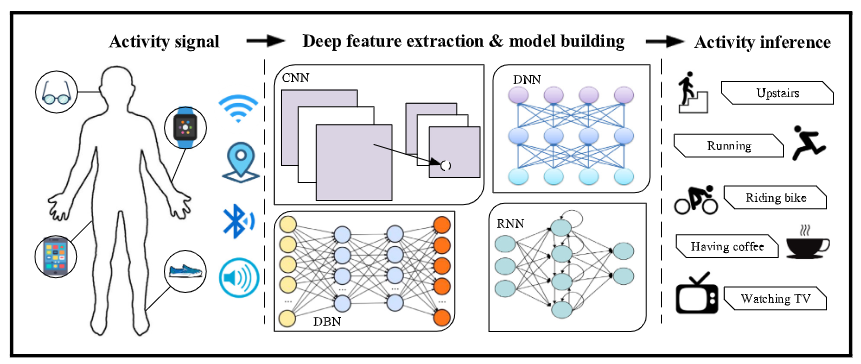
\includegraphics[width=0.9\textwidth]{content/2-Background/sensor-based-deep-learning.png}
    \caption[An illustration of sensor-based activity recognition using a machine learning approach]{An illustration of sensor-based activity recognition using a machine learning approach\cite{Wang2019b}.}
    \label{fig:back-sensor-based-deep-learning}
\end{figure}


% Types of machine learning models
Of the many machine learning types prevalent across the research field, \acrfull{cnn}, \acrfull{rnn} are the most common. Both are forms of neural network.

``\acrfull{cnn} are a specialised kind of neural network for processing data that has a known grid-like topology. Examples include time-series data taken at regular intervals and image data. \acrshort{cnn} have been tremendously successful in practical applications.''\cite{Goodfellow2015}

``\acrfull{rnn} are a family of neural networks for processing sequential data. \acrshort{rnn} specialised for processing a sequence of values. Can scale to much longer sequences than would be practical for networks without sequence-based specialism''\cite{Goodfellow2015} The most common form of \acrshort{rnn} used is the \acrfull{lstm}. This alleviates some of the issues with a base \acrshort{rnn} though additional methods of information flow control.

``We found that a Recurrent Neural Network (RNN) was the best performing model, robust to subject-specific variations such as walking speed and step length.''\cite{Rai2019a}


% Couple of examples of each type of network - ideally ones which talk about amputees
\acrshort{cnn} examples \cite{Martinez-Hernandez2021}

\acrshort{lstm} examples

Combined \acrshort{cnn} and \acrshort{lstm} - give example



%---------------------------------------------%
\section{Conclusions}
Tie all threads together

Powered prosthesis have different control modes to handles the needs of each different locomotive mode.

We need to be able to correctly identify the current activity mode that the user is trying to achieve so we can select an appropriate mode

Powered prosthesis already have a lot of sensors on board to measure the world around them such as IMUs. IMUs are a very good fit for the problem lets use more of them

heuristic hand-crafted is how mode selection is primarily done at the moment but this is time consuming and hard
Machine learning is a good fit for this converting raw sensor data into a classification of current gait mode

Limited research into human activity recognition for amputees using IMU data?
Probably because it's hard to collect data for amputees and machine learning requires a lot of data

So lets start with non-amputees
Apply learning from non-amputees to amputees!
Ideally use non-amputee data to improve the performance of an amputee classifier/reduce data requirements?